\documentclass[a4paper,14pt]{extarticle} \usepackage[utf8]{inputenc}
\usepackage[T1]{fontenc}
\usepackage[margin=2.5cm]{geometry}

% Fonte Caladea se existir, senão lmodern
\IfFileExists{caladea.sty}{
  \usepackage{caladea}
}{
  \usepackage{lmodern} }
\usepackage{ragged2e}
\usepackage{graphicx}
\usepackage[portuguese]{babel}
\usepackage{wrapfig}
\usepackage{hyperref}
\usepackage{fancyhdr}
\usepackage{xcolor}
\usepackage{rotating}
\usepackage{titlesec}
\usepackage{epigraph}
\usepackage{dirtytalk}
\usepackage{indentfirst} % Indenta o primeiro parágrafo após seções

% Ajuste do recuo de parágrafo
\setlength{\parindent}{1.5em}

% Adjust headheight to remove LaTeX warning
\setlength{\headheight}{17.54163pt}

% Centralizar títulos
\titleformat{\section}
  {\normalfont\centering\bfseries\Large}{}{1em}{}

\titleformat{\subsection}
  {\normalfont\centering\bfseries\large}{}{1em}{}

\titleformat{\subsubsection}
  {\normalfont\centering\bfseries}{}{1em}{}

% -------------- Símbolos de Versículo e Resposta --------------
% Definição do símbolo (a “barrinha” inclinada)
\makeatletter
\newcommand{\vers@resp@sym}{%
  \raisebox{0.2ex}{\rotatebox[origin=c]{-20}{$\m@th\rceil$}}%
}
% macro interna que sobrepõe a barrinha e a letra V ou R
\newcommand{\vers@resp}[2]{%
  {\ooalign{%
     \hidewidth\kern#1\vers@resp@sym\hidewidth\cr
     #2\cr
  }}%
}
% comandos públicos \versicle e \response
\DeclareRobustCommand{\versicle}{\vers@resp{-0.1em}{V}}
\DeclareRobustCommand{\response}{\vers@resp{0pt}{R}}
\makeatother
% ^------------- Símbolos de Versículo e Resposta -------------^

% Rodapé com imagem e página
\pagestyle{fancy}
% ---- Cabeçalho ------------
\fancyhf[C]{}
% ----- Rodapé --------------
\fancyfoot[C]{%
  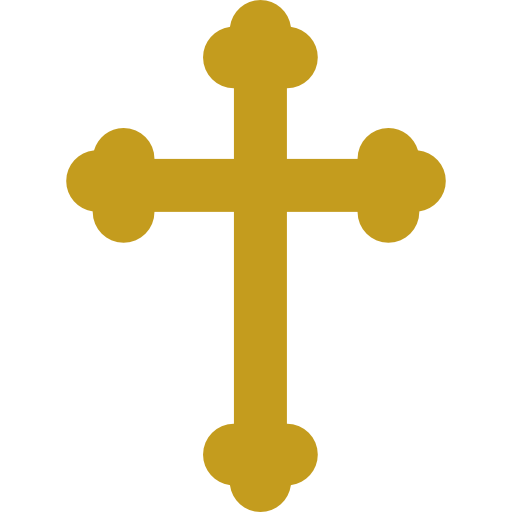
\includegraphics[scale=0.2]{assets/cross.png}\quad
  \textit{\textit{São João José da Cruz, Rogai por Nós}}\quad
  \thepage
}

\usepackage{pdfpages}
\begin{document}
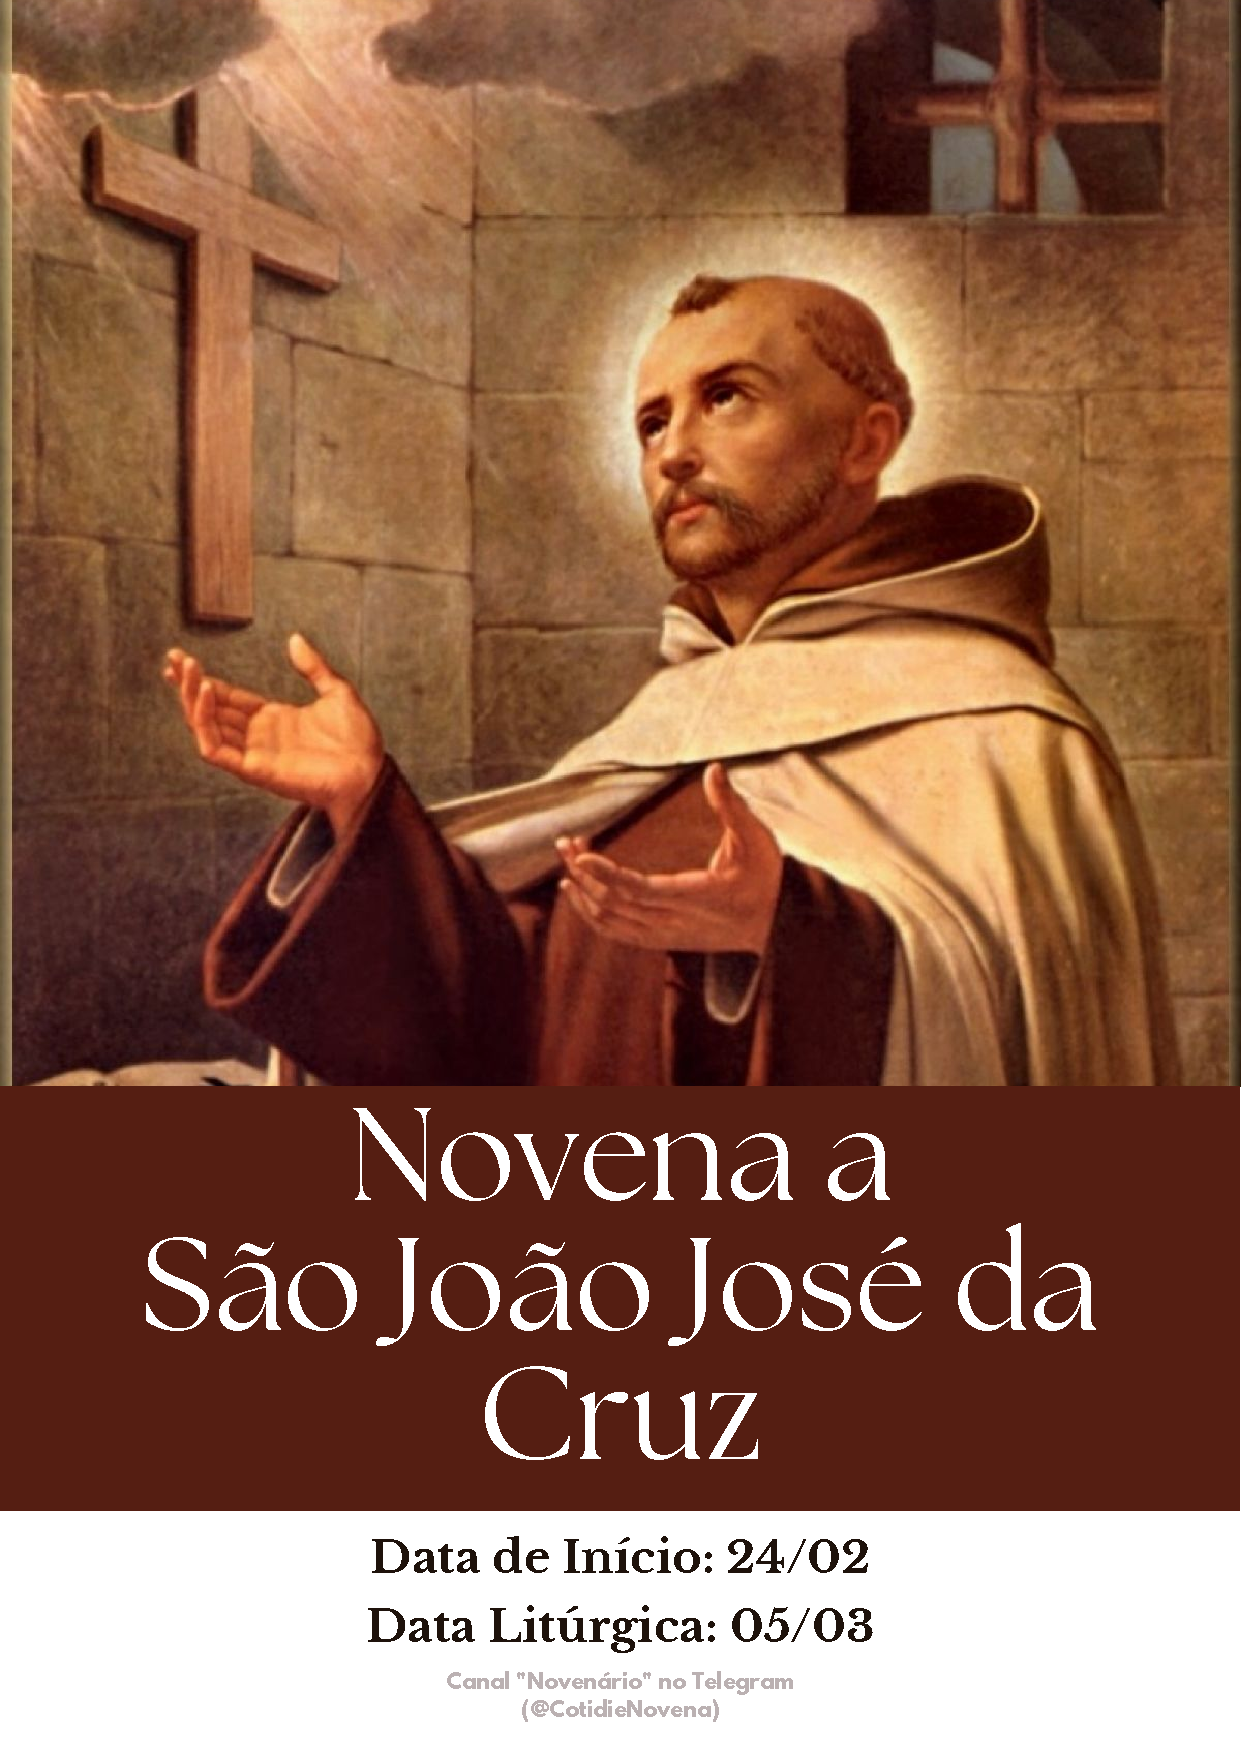
\includepdf[pages=1]{Capa São João José da Cruz}

\begin{center}
  {\huge Novena de São João José da Cruz}
\end{center}



\noindent\rule{\textwidth}{0.4pt}

\tableofcontents

\thispagestyle{empty}


% --- Origem ---
\newpage

\section{História}

São João José da Cruz, cujo nome de batismo é Carlos Caetano Calosinto, nasceu na Ilha de Isca, na Itália. Desde criança, em casa, já tinha uma grande devoção a Maria. Ao longo de sua vida, sempre invocava Nossa Senhora, buscando conselhos e conforto nas situações mais difíceis. Ele nasceu em uma família rica e religiosa e estudou com os agostinianos para aprofundar sua formação religiosa. Foi lá que o pequeno Carlos se apaixonou por Jesus e ouviu sua voz chamando-o para dedicar toda sua vida a Ele.
\subsection{Vocação ao despojamento}

Com apenas 16 anos, Carlos entrou para o convento de Santa Luzia no Monte, em Nápoles, onde mudou seu nome para João José da Cruz, no dia de sua profissão religiosa, aos 17 anos. Ele viveu entre os Frades Menores Descalços da Reforma de São Pedro de Alcântara, conhecidos como Alcantarinos. A regra mais austera dos Alcantarinos atraiu João José, que decidiu nunca usar sandálias. Essa busca pelo despojamento e simplicidade marcou toda sua vida.
\subsection{Devoção particular a Nossa Senhora}

João José tinha uma devoção especial a Nossa Senhora. Como Superior dos Alcantarinos, sempre manteve uma pequena imagem de Maria em sua escrivaninha, à qual contemplava e dirigia suas orações antes de qualquer decisão ou pronunciamento. Ele acreditava que não conseguia viver sem ela. Seus biógrafos e frades testemunham que ele recomendava prestar homenagem a Maria, pois através dela receberiam consolação, ajuda e luz para resolver os problemas. No leito de morte, suas últimas palavras sobre Maria foram: “Recomendo-lhe Nossa Senhora“, que pode ser considerado seu testamento espiritual.

\subsection{Amor à pobreza}

João José também mostrou um grande amor pela pobreza. Ele ia em busca dos pobres não apenas nas ruas, mas também nas favelas e casebres. Durante toda sua vida, usou apenas um hábito que com o tempo ficou todo remendado, o que lhe rendeu o apelido de “frade dos cem remendos”. Ele buscava imitar a Irmã Pobreza com perfeição e valorizava a simplicidade em sua vida, compartilhando o pouco que tinha com os mais necessitados.

\subsection{Fiel a São Pedro de Alcântara}


João José foi escolhido para fundar um novo mosteiro em Piedimonte e também construiu um pequeno eremitério chamado “A Solidão”, que até hoje é destino de peregrinações. Durante sua vida, teve que enfrentar a divisão entre os Alcantarinos da Espanha e da Itália. Como Provincial dos Alcantarinos da Itália, trabalhou por vinte anos para reunir novamente a família religiosa, mesmo enfrentando críticas injustas e calúnias. Ele foi muito fiel ao fundador da ordem, São Pedro de Alcântara, e contribuiu para restaurar a disciplina religiosa em muitos conventos na região napolitana.
Santificando-se e levando outros à santidade

João José faleceu em 5 de março de 1734, aos 80 anos. Ele foi canonizado por Gregório XVI em 1839, juntamente com Francisco de Jerônimo e Afonso Maria de Liguori, que o conheceram durante sua vida e buscaram seus conselhos. Durante sua vida, João José experimentou fenômenos místicos que demonstram o sopro especial da graça em sua vida, como bilocações, profecias, leitura dos corações, levitação, curas miraculosas e até mesmo uma ressurreição. No entanto, sua santidade e testemunho de vida ordinária falavam mais alto do que esses dons carismáticos.

% --- Orações Diárias ---
\newpage

\vfill

\section{Orações}
\subsection{Oração Inicial}\label{sub:inicial} % (fold)


Ó Deus, que concedestes a São João José da Cruz a graça de imitar Cristo na pobreza, na humildade e no amor à Cruz, dai-nos, por sua intercessão, a força para seguir os passos do Vosso Filho. Que ele, que brilhou pela fé inquebrantável e pela dedicação aos irmãos, nos inspire a viver uma vida de santidade.

Apresento-Vos, Senhor, as minhas intenções:
\textit{(coloque aqui suas intenções).}



\subsection{Dia 1 - A Humildade que Santifica}
\underline{\nameref{sub:inicial}}


São João José da Cruz renunciou às honras do mundo para seguir Cristo na simplicidade franciscana. Mesmo sendo superior, lavava os pés dos irmãos e servia aos mais pobres.
Ó São João José, que escolhestes a humildade como caminho para Deus, ensina-me a desprezar o orgulho e a servir com amor. Ajuda-me a encontrar na simplicidade a verdadeira alegria do Evangelho. Amém.

\underline{\nameref{sub:final}}


\subsection{Dia 2 - O Amor à Pobreza Evangélica}

\underline{\nameref{sub:inicial}}

São João José da Cruz abraçou a pobreza franciscana com radicalidade, vivendo apenas do necessário e repartindo tudo com os necessitados. Sua vida foi um testemunho de desapego.
Ó São João José, que amastes a pobreza como Cristo a amou, ajuda-me a libertar-me do apego aos bens materiais. Ensina-me a confiar na providência divina e a partilhar com os que sofrem. Amém.

\underline{\nameref{sub:final}}


\subsection{Dia 3 - A Devoção à Paixão de Cristo}


\underline{\nameref{sub:inicial}}

São João José meditava diariamente a Paixão de Cristo, unindo-se aos Seus sofrimentos. Ele via na Cruz a maior expressão do amor de Deus.
Ó São João José, que encontrastes na Cruz a força para a santidade, ajuda-me a amar os sofrimentos da vida como meio de purificação. Ensina-me a unir minhas dores às de Jesus pela salvação do mundo. Amém.


\underline{\nameref{sub:final}}


\subsection{Dia 4 - A Obediência à Vontade de Deus}


\underline{\nameref{sub:inicial}}

São João José da Cruz como superior, ele obedecia às regras com rigor, mas também com amor. Ensinava que a verdadeira liberdade está em seguir a vontade de Deus.
Ó São João José, que viveste a obediência com fidelidade, ajuda-me a discernir e acolher a vontade de Deus em minha vida. Dá-me a coragem de renunciar aos meus caprichos para seguir Cristo. Amém.


\underline{\nameref{sub:final}}


\subsection{Dia 5 - A Vida de Penitência}


\underline{\nameref{sub:inicial}}

São João José da Cruz jejuava frequentemente, dormia no chão e carregava cilícios para dominar o corpo e elevar a alma. Sua penitência era um ato de amor a Deus.
Ó São João José, que soubeste domar a carne para glorificar o espírito, ensina-me a praticar a mortificação com sabedoria. Ajuda-me a oferecer pequenos sacrifícios por amor a Cristo. Amém.


\underline{\nameref{sub:final}}


\subsection{Dia 6 - O Místico da Divina Luz}


\underline{\nameref{sub:inicial}}

São João José da Cruz teve visões e êxtases místicos, nos quais experimentava a presença de Deus de forma intensa. Sua vida de oração era a fonte de sua força.
Ó São João José, que mergulhastes na intimidade de Deus, ensina-me a rezar com fervor e constância. Ajuda-me a buscar a luz divina nas trevas da minha vida. Amém.


\underline{\nameref{sub:final}}


\subsection{Dia 7 - O Serviço aos Irmãos}


\underline{\nameref{sub:inicial}}

São João José da Cruz fundou mosteiros e guiou seus irmãos com sabedoria, sempre atento às necessidades espirituais e materiais de todos.
Ó São João José, que fostes um pai para os necessitados, ajuda-me a ser instrumento de paz e esperança. Ensina-me a servir sem esperar recompensa. Amém.


\underline{\nameref{sub:final}}


\subsection{Dia 8 - A Paciência nas Provações}


\underline{\nameref{sub:inicial}}

São João José da Cruz suportou calúnias, doenças e incompreensões com paciência heroica, confiando sempre na justiça divina.
Ó São João José, que aceitastes as cruzes da vida com serenidade, ajuda-me a suportar as provações com fé. Ensina-me a ver em cada dificuldade uma oportunidade de crescer no amor a Deus. Amém.


\underline{\nameref{sub:final}}


\subsection{Dia 9 - A Paciência nas Provações}

\underline{\nameref{sub:inicial}}

São João José da Cruz suportou calúnias, doenças e incompreensões com paciência heroica, confiando sempre na justiça divina.
Ó São João José, que aceitastes as cruzes da vida com serenidade, ajuda-me a suportar as provações com fé. Ensina-me a ver em cada dificuldade uma oportunidade de crescer no amor a Deus. Amém.

\underline{\nameref{sub:final}}


\subsection{Oração Final}\label{sub:final} % (fold) \subsection{Orações de Cada Dia}

\[\textbf{Pai-Nosso, Ave-Maria, Glória}\]

Ó Deus, que fizestes de São João José da Cruz um modelo de humildade, amor à Cruz e serviço aos irmãos, concedei-nos, por sua intercessão, a graça de imitar suas virtudes. Que ele, que tanto amou a pobreza e a oração, nos inspire a buscar a santidade em nossa vida cotidiana.

\vfill

\begin{center}
\subsection*{Fontes:}
Adaptado de: {\color{blue} \underline{\href{https://catolicoapp.com/santo/sao-joao-jose-da-cruz/}{Catolico App}}} e {\color{blue} \underline{\href{https://www.youtube.com/playlist?list=PLN7jQwkJvdQqUgkNY26QNpnL5zagNNgRU}{Canal A Oração dos Santos}}}
\end{center}


\end{document}
